\section{Rekursion}

\subsection*{(a) $f(n)$}

Vi vil vise, at antallet af ord $f(n)$ med længden $n$ bogstaver, som følger de givne regler i opgavesættet, er givet ved:
\[ f(n) = \begin{cases} 
      0 & n < 0 \\
      1 & n = 0 \\
      2 f(n-1) + 2 f(n-2) & n > 0
   \end{cases}
\]
\\

Vi betragter først basistilfældene $n<0$ og $n=0$.\\
\\
$n<0$: Det er ikke muligt at lave ord med et negativt antal bogstaver, så $f(n)=0$ for $n<0$.\\
$n=0$: Der er kun én måde, vi kan lave et ord med 0 bogstaver, nemlig ved ikke at bruge nogen bogstaver. Så $f(0)=0$.\\
\\
$n>0$: Vi betragter et vilkårligt legalt ord med $n>0$ bogstaver, der ender på $a$ eller $b$. Vi skriver det som
\begin{equation}
    [\quad]_0 \, ... \, [\quad]_{n-2} \, [\quad]_{n-1} \, [a/b]_n, 
\end{equation}

hvor kantede parenteser repræsenterer et bogstav, og sænket skrift repræsenterer bogstavet indeks. Det sidste bogstav læses "$a$ eller $b$". Vi forestiller os, at vi fjerner det $n$'te bogstav. Er ordet med $(n-1)$ bogstaver et legalt ord?\\
\\
\textcolor{red}{\textbf{Case 1}} og \textcolor{blue}{\textbf{Case 2}}: Hvis det $(n-1)$'te bogstav er $a$ eller $b$, og alle forrige bogstaver overholder reglerne, er det $(n-1)$'te ord legalt. Efter at have fjernet det $n$'te $a$ (eller $b$), er vi tilbage til start: vi har et legalt ord med $(n-1)$ bogstaver, der slutter med $a$ eller $b$.\\
\\
\textcolor{orange}{\textbf{Case 3}} og \textcolor{black}{\textbf{Case 4}}: Hvis det $(n-1)$'te bogstav er et $c$, er ordet med $(n-1)$ bogstaver ikke legalt. Men hvis det $(n-2)$'te bogstav er et $a$ eller $b$, og alle de forrige bogstaver overholder reglerne, er ordet med $(n-2)$ bogstaver et legalt ord. Efter at have fjernet det $n$'te $a$ (eller $b$) og det $(n-1)$'te $c$, er vi tilbage til start: vi har et legalt ord med $(n-2)$ bogstaver, der slutter med $a$ eller $b$.

\begin{figure}[H]
\centering
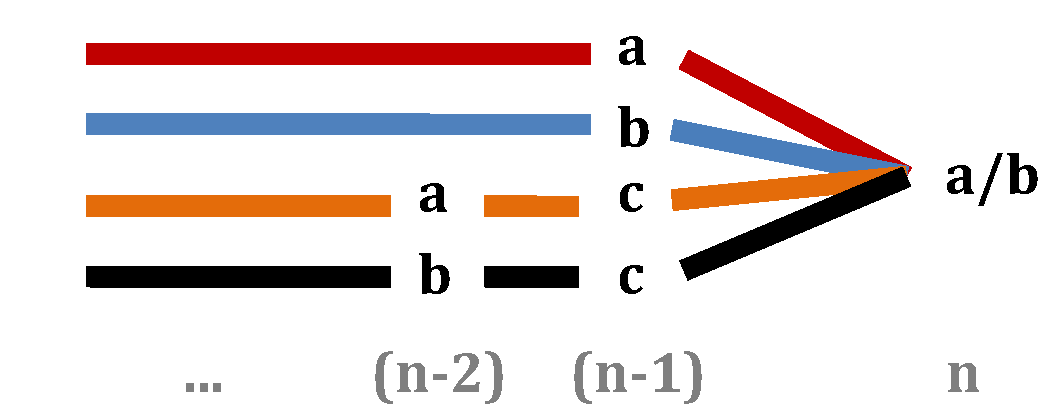
\includegraphics[width=0.7\textwidth]{Opg2/fig/2a.pdf}
\caption{Visualisering af legale ord. Rækkefølgen af bogstaver er $(n-2) \quad (n-1) \quad n$.}
\label{fig:2a}
\end{figure}

Der findes således \textcolor{red}{$f(n-1)$} legale ord, der slutter med $a$ og er ét bogstav kortere end $[\quad]_0 \, ... \, [\quad]_{n-2} \, [\quad]_{n-1} \, [a/b]_n$. Der findes også \textcolor{blue}{$f(n-1)$} legale ord, der slutter med $b$ og er ét bogstav kortere.\\
\\
Der findes \textcolor{orange}{$f(n-2)$}+\textcolor{black}{$f(n-2)$} legale ord, der er to bogstavere kortere end \\
$[\quad]_0 \, ... \, [\quad]_{n-2} \, [\quad]_{n-1} \, [a/b]_n$.\\

Så hvor mange legale ord kan vi skrive med $n$ bogstaver?
\begin{equation}
f(n) = \textcolor{red}{f(n-1)} + \textcolor{blue}{f(n-1)} + \textcolor{orange}{f(n-2)}  + \textcolor{black}{f(n-2)} = 2 f(n-1) + 2 f(n-2)
\end{equation}

som ønsket.

\subsection*{(b) $f(4)$}
$f(-1)=0$ og $f(0)=1$ ifølge definitionen. Vi beregner $f(n)$ og $n!$ for udvalgte værdier. $f(n)$ beregnes ved 2 gange summen af de to forrige elementer:
\begin{equation}
f(n) = 2 f(n-1) + 2 f(n-2) = 2 \left( f(n-1) + f(n-2) \right)
\end{equation}

\renewcommand{\arraystretch}{1.3}
\begin{table}[H]
\begin{center}
    \begin{tabular}{ccccccccc}
    \hline
    $n$    & $-$1 & 0 & 1 & 2 & 3  & 4  & 5   & 6   \\ \hline
    $f(n)$ & 0  & 1 & 2 & 6 & 16 & 44 & 120 & 328 \\ \hline
    $n!$   &   & 1 & 1 & 2 & 6  & 24 & 120 & 720 \\ \hline
    \end{tabular}
    \vspace{-0.5cm}
    \caption{Udvalgte værdier af $f(n)$ og $n!$.}
    \label{tab:2b}
    \end{center}
\end{table}
\renewcommand{\arraystretch}{1.0}

Dvs. $f(4)=44$.

\subsection*{(c) $f(n) < n!$}
Det ses i tabel \ref{tab:2b} at $f(n) < n!$ for $n=6$. Så der findes et $n \in \mathbb{N}$ således at $f(n) < n!$.\\
\\
Man kan undersøge højere værdier for $n$. Det viser sig at for alle $n \geq 6$ er $n! > f(n)$ da $\frac{f(n+1)}{f(n)}$ konvergerer mod $2.73205$ (undersøgt med WolframAlpha) for $n \rightarrow \infty$, mens $\frac{(n+1)!}{n!}$ divergerer for $n \rightarrow \infty$. Opgaven spurgte dog kun om der findes ét $n$.